\section{Pedestrian Dead Reckoning (PDR)} \label{sec:pdr}

\gls{pdr} is a positioning method, where the traveled distance and a heading are added to the known starting position \cite{pdr_smartphonebased}. The \gls{pdr} method is described in \cite{HybridPositioningPaper} and uses the \gls{imu} for positioning. The tracking of the pedestrian can be accomplished through performing step detection, step length estimations and heading estimation. Tracking a pedestrian is done in iterations, where computing a position is based on the previous position computed.

As seen in many papers, such as in \cite{pdr_smartphonebased, HybridPositioningPaper, 6987239, 6782540}, \gls{pdr} is a common solution for position estimation, and we have therefore chosen to experiment with this method. Our method is constructed with inspiration from multiple works. A graphical presentation of the method is shown in \textbf{\autoref{fig:pdr}}. The Z-axis dispersion and step detection is acquired from \cite{peakdetection}, and the step length estimation is from \cite{HybridPositioningPaper}. For the heading estimation, the toolkit \gls{ahrs} is used, where different filters from the toolkit have been researched. The different components of the method will be elaborated further on in the following sections. Each of the components have a dedicated number from 1 to 5 to make the process easier to explain. 
\\

\begin{figure}[H]
    \centering
    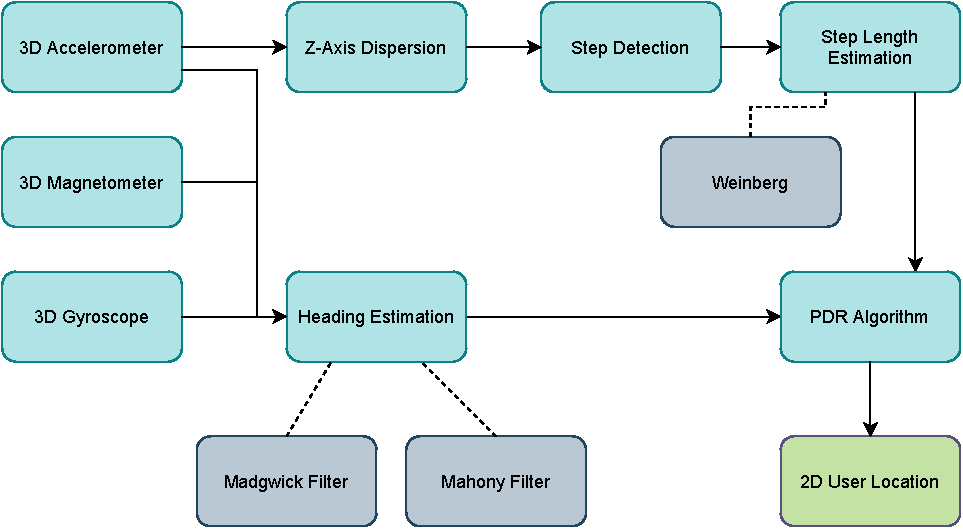
\includegraphics[scale=0.7]{Images/Experiments/pdr.pdf}
    \caption{PDR implementation architecture.}
     \label{fig:pdr}
\end{figure}

% Tag elementer fra filen geometry_based.tex fra 1.Problem_analysis til forklaring af PDR.

\subsection{Step Detection}

The general idea of step detection of a pedestrian with a smartphone is by measuring the accelerometer sensor and observe the increases and decreases in the acceleration pattern\cite{HybridPositioningPaper}. We have chosen to follow the algorithm proposed in \cite{peakdetection}. This is due to the fact that it is the only solution implementable for smartphones in a walking scenario.

The algorithm is based on the principle of dispersion, which is the extent to which a distribution is stretched or squeezed \cite{dispersion}. As seen in figure \textbf{\autoref{fig:pdr}}, the Z-axis dispersion is computed before the step detection. This step includes smoothening of the data to remove noise. This is included in the first step in \textbf{\autoref{fig:pdr}}, which is denoted by the number \textbf{1}.

For the step detection, which is \textbf{step 2} in \textbf{\autoref{fig:pdr}}, the algorithm will return a signal value if a new datapoint is a specific amount of deviations away from a moving mean. This amount of deviations is also called the z-score. The algorithm creates a separate moving mean and deviation, and signals can therefore not corrupt the threshold. The algorithm takes 3 inputs: \textit{lag}, \textit{threshold} and \textit{influence}. \textit{Lag} determines how much the input data is to be smoothened. Therefore, low lag values result in the algorithm being quicker at adapting to the input data. Since the input data for step detection vary a lot, the lag value will be low. The \textit{threshold} is the z-score at which the algorithm will return a signal. Lastly, the \textit{influence} is the impact of new signals on the mean and deviation. The influence can be between 0 and 1. If 0 is chosen as the influence, signals would be completely ignored for recalculation of a new threshold. This choice would assume stationarity, meaning that the statistical properties of a process, such as the mean, variance and the structure of the autocorrelation, do not change over time\cite{stationarity}. In our case, we are working with data from walking people in a shopping mall. Since random walking is not a stationary process, we will use a nonzero value\cite{peakdetection}. The \textit{threshold} value is set to 10, since this is the value we deemed as giving the best result for detecting steps for our data set by trial-and-error. The \textit{threshold} value is found by using a subset of the data provided by Indoor Location \& Navigation Competition from Kaggle that corresponds to a single step to evaluate when the algorithm signals a step. The \textit{lag} value is set to 2, and is found in the same way as the \textit{threshold} value.

\subsection{Step Length Estimation}

For step length estimation, there exists two methods: static and dynamic. The static method assumes a person is walking at a constant velocity, whereas the dynamic method makes use of an accelerator for dynamic estimation. Weinberg is one method for dynamic step length estimation. We have decided to use the Weinberg method due to its low error compared to other methods \cite{HybridPositioningPaper}. This is executed in \textbf{step 3} in \textbf{\autoref{fig:pdr}}.  

The Weinberg method is defined in \textbf{\autoref{eq:weinberg}}\cite{weinberg}.

\begin{equation} \label{eq:weinberg}
    l = k \sqrt[4]{a_{LPF, peak} - a_{LPF, valley}}
\end{equation}

In \textbf{\autoref{eq:weinberg}}, $k$ is a constant factor for unit conversion, $a_{LPF, peak}$ is the maximum acceleration in the z-axis and $a_{LPF, valley}$ is the minimum acceleration in the z-axis. The value $k = 0.5$ is used in \cite{HybridPositioningPaper}, and we also found that this value yielded the best result by error-and-trial.

\subsection{Heading Estimation}
\textbf{Step 4} is the heading estimation. The heading estimation is accomplished using \gls{ahrs}, which is a Python toolkit for estimation attitude containing several functions and utilities for the attitude estimations\cite{ahrs, FastAHRS}. According to \cite{MultisensorComparison}, Madgwick and Mahony perform best in comparison to other alternative algorithms, both of which are provided by \gls{ahrs}. But since Madgwick outperforms Mahony according to \cite{Ludwig2018ComparisonOA}, we have decided to experiment with Madgwick. The Extended Kalman Filter is also implemented because of it being one of the most widely used algorithms\cite{ahrs}. Both of these algorithms compute a set of quaternions, given a set of acceleration data and gyroscope data, from which a heading can be computed. Quaternions is a way of representing 3D rotations\cite{quaternion_math}.

\subsection{Position Estimation}

\textbf{Step 5} is the last step before achieving the 2D user location using equations \textbf{\autoref{eq:pdr_X}} and \textbf{\autoref{eq:pdr_Y}}.

\begin{equation} \label{eq:pdr_X}
    x_t = x_{t - 1} + l_t\cos(\theta_t)
\end{equation}

\begin{equation} \label{eq:pdr_Y}
    y_t = y_{t - 1} + l_t\sin(\theta_t)
\end{equation}

\textbf{\autoref{eq:pdr_X}} and \textbf{\autoref{eq:pdr_Y}} are the central equations to compute in order to estimate a location $(x_t, y_t)$ at time $t$, given a previous location $(x_{t - 1}, y_{t - 1})$, a step length $l_t$ and a heading $\theta_t$ in radian.